% main.tex -- draft manuscript, prepared by claude-interactive.20 (claude-opus-5-5, claude), 2026-10-19,
% task T-20261019-claude-interactive.20-01. Build with ./build.sh. Every number cites a run id under runs/
% (figure captions, text and the provenance table of Appendix G).
\documentclass[aps,pra,twocolumn,superscriptaddress,nofootinbib,floatfix]{revtex4-2}
\usepackage[T1]{fontenc}
\usepackage{amsmath}
\usepackage{newtxtext,newtxmath}
\usepackage{graphicx}
\usepackage{xcolor}
\usepackage[colorlinks=true,linkcolor={blue!45!black},citecolor={blue!45!black},urlcolor={blue!45!black}]{hyperref}
\usepackage{xurl}
\hypersetup{pdftitle={Quantum noise around the amplifier similariton},
  pdfauthor={Authors to be set by the PI; draft by claude-interactive.20 (Claude Opus 5.5)}}

\newcommand{\LNL}{L_{NL}}
\newcommand{\PNL}{\Phi_{NL}}
\newcommand{\nsp}{n_{sp}}
\newcommand{\Nout}{N_{\rm out}}
\newcommand{\eps}{\varepsilon_0}
\newcommand{\lamLO}{\lambda_{\rm LO}}
\DeclareRobustCommand{\run}[1]{{\small\path{#1}}}
\newcommand{\rk}[1]{[\textsf{#1}]}

\begin{document}

\title{Quantum noise around the amplifier similariton:\\
phase-sensitive shape modes, energy--phase locking and the limits of matched-mode squeezing}

\author{Authors: to be set by the PI}
\noaffiliation

\date{Draft, October 19, 2026}

\begin{abstract}
A pulse amplified in a fibre with normal dispersion is attracted to a parabolic similariton. We collect analytical
results on the quantum noise of this process, each checked by an independent implementation written by a second model
family. In the leading, dispersionless theory every Legendre shape mode $\ell\ge2$ acts as a phase-sensitive amplifier:
photon-normalized intensity- and phase-shape variances grow as $G^{1/3}$ and $G^{5/3}$ with the power gain $G$, against
$G$ for a linear amplifier, with prefactors that oscillate in $\ln G$. Two measurable projections therefore collapse onto
the energy fluctuation: a five-component projection of the single-shot spectral covariance has eigenvalue ratio
$\mu_2/\mu_1=\Theta(G^{-2/3})$, and the phase quadrature of a matched local oscillator becomes energy-locked with
deficit $1-r^2=\Theta(G^{-2/3})$, while its variance grows as $(32n_{sp}/9)G\Phi_{NL}^2\propto G^{7/3}$. Amplifier
noise does not forbid squeezing: at short length the matched mode is squeezed despite full spontaneous emission when
$\gamma\int P^2/\int P>n_{sp}g$. At large gain its minimum variance grows as $G^{1/3}$. We give the steps that carry each
derivation, the regime as bounds on dimensionless groups, what failed in verification, and what to measure.
\end{abstract}

\maketitle

%=====================================================================================================
\section{Introduction}

A pulse amplified in a normally dispersive fibre approaches a parabolic similariton, whose width grows as $G^{1/3}$
and whose chirp is linear~\cite{fermann2000,kruglov2002,finot2004}; the parameter dynamics of this attraction are
published~\cite{wabnitz2007,wabnitz2007qels}. Its noise has been computed numerically for similariton
lasers~\cite{zweck2018} and measured as classical intensity noise of the total power at one gain, without quantum, phase
or shape-resolved noise~\cite{wang2016spie,wang2016ol}, or in spectral slices~\cite{haviv2026}. We collect analytical results on the quantum noise of single-pass similariton
amplification: how the attraction reshapes vacuum and amplified spontaneous emission (ASE) in the low-order shape modes
(Sec.~\ref{sec:shape}), what this does to two measurable projections, the single-shot spectrum and a matched local
oscillator (LO) (Sec.~\ref{sec:proj}), and when the matched mode can be squeezed despite phase-insensitive gain
(Sec.~\ref{sec:sq}). For each statement we give the steps that carry it, its regime and how it was checked.

The statements are two results of the project repository at its ``promising'' tier, R-0011 and R-0014
(Table~\ref{tab:status}). Each was proposed by one model family and verified with independent code written by
another; R-0011 also passed a clean-context audit. Neither is formalized or peer reviewed. Two statements of the
original claim failed and are reported as failures.

The ingredients are known: the hydrodynamic modes of a parabolic (Thomas--Fermi) condensate, with spectrum
$\propto\ell(\ell+1)$~\cite{menotti2002}, and the separation of fluctuations on an expanding background~\cite{fedichev2004};
the quantum limit of linear amplifiers~\cite{caves1982} and the Langevin theory of fibre noise~\cite{drummond2001}; Kerr
conversion of amplitude noise into phase noise~\cite{gordon1990} and its correction from measured
intensity~\cite{ho2004}; pulsed Kerr squeezing read with a pulse-matched LO~\cite{shirasaki1990,doerr1994}. Linearizing
the published width equation already gives the decay of the breathing ($\ell=2$) mode at rate $g/3$, so that rate is not
new. Bounded searches by agents of both families did not find the noise exponents, the spectral and phase--energy laws or the
short-length squeezing criterion; a two-mode Kerr amplifier with a related noise advantage has been proposed outside
fibres~\cite{ren2026}. These searches do not establish novelty.

%=====================================================================================================
\section{Model and scales}\label{sec:model}

We use the scalar nonlinear Schr\"odinger equation with flat, unsaturated power gain $g$ and its Langevin noise,
\begin{equation}
\partial_zA=-\tfrac{i\beta_2}{2}\partial_T^2A+i\gamma|A|^2A+\tfrac g2A+F,\label{eq:nlse}
\end{equation}
with $\beta_2>0$, $|A|^2$ in photons per unit time, $\langle F^\dagger F\rangle=g\nsp\delta$ and
$\langle FF^\dagger\rangle=g(\nsp-1)\delta$, $\delta=\delta(z-z')\delta(T-T')$; this reservoir keeps the commutator.
The seed is a coherent state of $N_0$ photons, $G=e^{gz}$, $\tau=\ln G$ and $\Nout=GN_0$. The noise is linearized about
the bright mean field.

With $L_D=T_0^2/\beta_2$ and $\LNL=1/(\gamma P_0)$ the groups are $\eps=\sqrt{\LNL/L_D}$ and $\Gamma=g\sqrt{L_D\LNL}$;
$\zeta=z/\sqrt{L_D\LNL}$, so $\tau=\Gamma\zeta$, and $x=T/T_0$. At leading order in $\eps$ the intensity $\rho$ and the
velocity $v=-\eps\partial_x\phi$ obey $\rho_\zeta+(\rho v)_x=\Gamma\rho$ and $v_\zeta+vv_x=-\rho_x$. The parabola
$\bar\rho=\rho_{\rm pk}(1-\xi^2)$, $\bar v=a'x/a$, with comoving time $\xi=x/a$, is an exact solution if $a''=2e^{\Gamma\zeta}/a^2$
(unit peak and half-width at launch); its asymptote is $a=A_*e^{\tau/3}$ with $A_*^3=18/\Gamma^2$. The peak nonlinear phase
$\PNL=\int\gamma P_{\rm pk}\,dz$ is $\frac{3}{2\Gamma A_*\eps}(G^{2/3}-1)$ on the asymptote, and the local semiclassical
parameter $\varepsilon_{\rm eff}=\eps/\sqrt{ae^{\Gamma\zeta}}$ falls as $G^{-2/3}$.

Fluctuations are written $\delta|A|^2=\rho_{\rm pk}n(\xi)$ and $\delta\arg A=p(\xi)$, with Legendre components $n_\ell$,
$p_\ell$. Quadratures have vacuum covariance $I$. The matched LO is the output mean field. It reads the number quadrature
$X_A=\delta N/\sqrt N$ and the phase quadrature $P_{\rm LO}=2\sqrt N\,\bar p$, where $\bar p=p_0-p_2/5$ is the
intensity-weighted mean phase; $C_{AA}$, $C_{PP}$, $C_{AP}$ is their covariance $C_{\rm LO}$ and $r$ their correlation.
The linearization needs the phase noise to be small, $\PNL^2/N_0\ll1$, which is not uniform in gain.

Numbers are cited by run: \rk{P}~\run{2026-10-18-pi-chatgpt-independent-verification} (GPT 6 Pro);
\rk{E}~\run{2026-10-19-gpt-e-similariton} (gpt-e); \rk{V}~\run{2026-10-19-claude-interactive.13-similariton-lo-verification}
(claude-interactive.13); \rk{A}~\run{2026-10-11-gpt-a-highlights-audit-c2} (gpt-a);
\rk{Q}~\run{2026-10-19-claude-interactive-gpt6pro-quick-repro} (claude-interactive);
\rk{S}~\run{2026-10-08-claude-a-amp-sim-checks} (claude-a). Appendix~\ref{app:prov} lists each number with its run and agent.

%=====================================================================================================
\section{Shape modes are amplified phase-sensitively}\label{sec:shape}

\textit{Statement} (R-0011a). For every fixed $\ell\ge2$ and input vacuum plus ASE, in leading parabolic hydrodynamics on
the asymptote,
\begin{equation}
\Nout{\rm Var}\,n_\ell=\Theta(G^{1/3}),\qquad \eps^2\Nout{\rm Var}\,p_\ell=\Theta(G^{5/3}),\label{eq:shape}
\end{equation}
against $\Theta(G)$ for both quadratures of a linear amplifier. $\Theta$ means bounded above and below by positive
constants times the power; the prefactors oscillate in $\ln G$, so they need not converge.

\textit{Crux.} Linearize about any parabolic background at fixed $\xi$. The gain term cancels against the growth of
$\rho_{\rm pk}$, the phase is carried along the background flow, and the pressure term becomes Legendre's operator,
$\partial_\xi[(1-\xi^2)\partial_\xi]P_\ell=-\ell(\ell+1)P_\ell$, as for the modes of a one-dimensional Thomas--Fermi
condensate~\cite{menotti2002,fedichev2004}. Each component then evolves on its own:
\begin{equation}
\frac{dp_\ell}{d\zeta}=\frac{e^{\Gamma\zeta}}{a}\frac{n_\ell}{\eps},\qquad
\frac{d}{d\zeta}\frac{n_\ell}{\eps}=-\frac{\ell(\ell+1)}{a^2}\,p_\ell .\label{eq:block}
\end{equation}
Eliminating $p_\ell$ on the asymptote gives, with $'=d/d\tau$,
\begin{equation}
n_\ell''+\tfrac23n_\ell'+\tfrac{\ell(\ell+1)}{18}n_\ell=0,\label{eq:legendre}
\end{equation}
with roots $\frac13[-1\pm\sqrt{1-\ell(\ell+1)/2}]$: the energy ($\ell=0$) is neutral, $\ell=1$ is a double root, and every
$\ell\ge2$ decays as $G^{-1/3}$ while oscillating at $\nu_\ell=\frac13\sqrt{\ell(\ell+1)/2-1}$ in $\ln G$ ($\nu_2=\sqrt2/3$).
By Eq.~\eqref{eq:block}, $p_\ell'\propto e^{2\tau/3}n_\ell/\eps$, so the phase response grows as $G^{1/3}/\eps$. In the
coordinates $u_\ell=G^{1/3}n_\ell$, $w_\ell=\eps G^{-1/3}p_\ell$ the drift is a constant matrix $B_\ell$ with
$B_\ell^2=-\nu_\ell^2I$, and the propagator is a bounded rotation. Noise enters $n_\ell$ with variance
$\propto1/N(\tau)\propto e^{-\tau}$, which is $e^{-\tau/3}$ in $u_\ell$: vacuum and early ASE dominate, and the covariance
of $(u_\ell,w_\ell)$ tends to a bounded, positive, oscillating matrix. Undoing the scaling, ${\rm Var}\,n_\ell\sim G^{-2/3}/N_0$
and ${\rm Var}\,p_\ell\sim G^{2/3}/(\eps^2N_0)$; multiplying by $\Nout=GN_0$ gives Eq.~\eqref{eq:shape}. Relative to linear
amplification, the attraction de-amplifies intensity-shape noise by $G^{-2/3}$ and amplifies phase-shape noise by
$G^{2/3}$. This contraction is not squeezing below vacuum.

\begin{figure}[t]
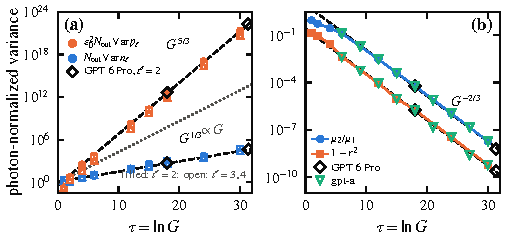
\includegraphics[width=\columnwidth]{figures/fig1_shape.pdf}
\caption{Shape-mode noise in the reduced model ($\Gamma=\sqrt{18}$, $\nsp=1$, seed on the asymptote). (a) Photon-normalized
intensity (blue) and phase (orange) variances of the orthonormal Legendre components $\ell=2$ (filled), 3, 4 (open); dashed:
$G^{1/3}$, $G^{5/3}$; dotted: $\propto G$, a linear amplifier. (b) Eigenvalue ratio $\mu_2/\mu_1$ of the five-component
spectral covariance and phase--energy deficit $1-r^2$; dashed: $G^{-2/3}$. Coloured symbols: gpt-e's clean-context
integration, run \run{2026-10-19-gpt-e-similariton}. Diamonds: GPT 6 Pro at equal phases of the oscillation,
\run{2026-10-18-pi-chatgpt-independent-verification}. Triangles: gpt-a, \run{2026-10-11-gpt-a-highlights-audit-c2}.}
\label{fig:shape}
\end{figure}

\textit{Checks.} In GPT 6 Pro's finite-volume covariance code (family gpt) the fitted powers over $12\le\tau\le26$ are
0.32461 and 1.69203; fits between equal phases of the oscillation give 0.33349 and 1.66676 \rk{P}. In gpt-e's
clean-context integration (gpt) the compensated $\ell=2$ variances $G^{-1/3}\Nout{\rm Var}\,n_2$ and
$G^{-5/3}\eps^2\Nout{\rm Var}\,p_2$ stay within [1.11, 2.68] and [0.186, 0.447] for $12\le\tau\le30$ \rk{E}
[Fig.~\ref{fig:shape}(a)]. The full NLSE, with all dispersive terms, a rounded asymptotically chirped seed, vacuum and
both ASE quadratures, gives an $\ell=2$ decay rate 0.333825 and log-gain frequency 0.470401 (predicted $1/3$ and 0.471405)
over $1\le\tau\le6$ at $\eps=0.05$; doubling the grid and halving the step change the rate by $2\times10^{-10}$ \rk{P}.
gpt-a's full-field rates are 0.33316, 0.33375 and 0.33259 for $\ell=2$, 3, 4 \rk{A}. No full-NLSE noise computation exists
for $\tau\ge12$.

%=====================================================================================================
\section{Spectral rank one and energy--phase locking}\label{sec:proj}

\subsection{Single-shot spectrum}

The output is strongly chirped, so a dispersive Fourier transform maps time to frequency, $\omega\simeq\kappa T$ with
$\kappa=\dot T_p/(\beta_2T_p)$. Let $s=\delta S/S_0$, with $S_0$ the peak of the mean spectrum and Legendre components $s_\ell$
over the spectral core, and let $\mu_1\ge\mu_2$ be the largest eigenvalues of the covariance of $(s_0,\dots,s_4)$ in the
orthonormal $L^2[-1,1]$ metric.

\textit{Statement} (R-0011b). On the asymptote $\mu_2/\mu_1=\Theta(G^{-2/3})$, for this five-component projection.

\textit{Crux.} Stationary phase gives $s_\ell=n_\ell-\ell(\ell+1)\eps p_\ell/(aa')$, which on the asymptote is
$s_\ell=n_\ell+3n_\ell'$. The energy component $s_0=\frac23\delta N/N$ is fixed once injected, while
$s_{\ell\ge1}=O(G^{-1/3})$; for $\ell=1$ the secular term cancels, since $n_1=(c_1+c_2\tau)e^{-\tau/3}$ gives
$s_1=3c_2e^{-\tau/3}$. The covariance therefore has the block form
\begin{equation}
C_s=\begin{pmatrix}c_0&G^{-1/3}b^{\mathsf T}\\ G^{-1/3}b&G^{-2/3}D\end{pmatrix},\label{eq:schur}
\end{equation}
and if $c_0>0$ and the Schur complement $D-bb^{\mathsf T}/c_0$ stays positive and bounded, $\mu_1=c_0+O(G^{-2/3})$ while
$\mu_2=\Theta(G^{-2/3})$. The single-shot spectral noise collapses onto the energy fluctuation. This is not a statement
about the full field, nor one that the quantum state becomes rank one.

\subsection{Matched local oscillator}

\textit{Statement} (R-0011c, R-0014i). In the reduced model on the asymptote,
\begin{gather}
C_{AA}=2\nsp G-(2\nsp-1),\label{eq:caa}\\
C_{PP}=\tfrac{32\nsp}{9}\,G\,\PNL^2\,\big[1+O(G^{-1/3})\big]\propto G^{7/3}/\eps^2,\label{eq:cpp}\\
1-r^2=\Theta(G^{-2/3}).\label{eq:r2}
\end{gather}

\textit{Crux.} Equation~\eqref{eq:caa} is exact in the linearized theory, for any pulse and dispersion: Kerr and
dispersion conserve photon number, so $X_A=\delta N/\sqrt N$ sees only the gain and its reservoir, a linear amplifier. The
phase follows from the $\ell=0$ block, $p_0'=\PNL'n_0$, where $n_0=\frac23\delta N/N$ changes only by ASE kicks $dW_0$ of
variance $\propto e^{-\tau}d\tau/N_0$. Integrating by parts,
\begin{equation}
p_0=\PNL n_0+R_0,\qquad R_0=-\textstyle\int_0^\tau\PNL\,dW_0 .\label{eq:regress}
\end{equation}
The first term has variance $\PNL^2{\rm Var}\,n_0\to\frac{8\nsp}{9}\PNL^2/N_0$, of order $G^{4/3}/(\eps^2N_0)$; the
residual has ${\rm Var}\,R_0\propto\eps^{-2}\int^\tau e^{4\tau'/3}e^{-\tau'}d\tau'/N_0=O(G^{1/3}/\eps^2N_0)$. With $C_{PP}=4\Nout{\rm Var}\,\bar p$
this gives Eq.~\eqref{eq:cpp}; the leading correction is the $p_0$--$p_2$ cross-covariance, $\Theta(G)$ against
$\Theta(G^{4/3})$. The part of $\bar p$ not linear in the energy is dominated by the shape phase $p_2/5$, whose conditional
variance is $\Theta(G^{2/3}/\eps^2N_0)$ by Sec.~\ref{sec:shape}; dividing by the total gives Eq.~\eqref{eq:r2},
independent of $\eps$. The phase noise is the Gordon--Mollenauer conversion of energy noise~\cite{gordon1990},
accumulated over a nonlinear phase that itself grows as $G^{2/3}$. The original claim's $C_{PP}\propto G/\eps^2$
contradicted its own $\ell=0$ formula and is superseded.

\begin{figure}[t]
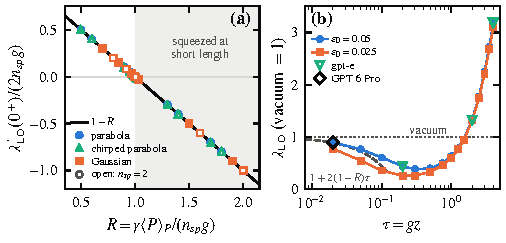
\includegraphics[width=\columnwidth]{figures/fig2_short.pdf}
\caption{Squeezing of the matched mode at short length despite full ASE. (a) Initial slope of the matched-mode minimum
variance, divided by $2\nsp g$, against $R$; line: Eq.~\eqref{eq:slope}. Smoothed parabolas (unchirped and chirped) and a
Gaussian; open symbols: held-out $\nsp=2$. (b) $\lamLO$ against $\tau$ in the full field ($\Gamma=\sqrt{18}$, $\nsp=1$;
parabola smoothed at $\delta=0.05$, with the asymptotic chirp), vacuum and both reservoir quadratures included; dashed:
first order, $1+2(1-R)\tau$ with $R=3.76$ for $\eps=0.05$. Lines: run
\run{2026-10-19-claude-interactive.13-similariton-lo-verification}. Triangles: gpt-e, chirped unsmoothed launch,
$\eps=0.05$, \run{2026-10-19-gpt-e-similariton}. Diamond: GPT 6 Pro's counterexample on its own launch,
\run{2026-10-18-pi-chatgpt-independent-verification}.}
\label{fig:short}
\end{figure}

\textit{Checks.} Reduced model: fitted powers $-0.66551$ (spectral ratio) and $-0.65351$ (deficit) over $12\le\tau\le26$,
and $-0.66734$ for the deficit between equal phases \rk{P}. Three gpt-family implementations agree, for example
$\mu_2/\mu_1=3.03\times10^{-3}$ and $1-r^2=8.96\times10^{-5}$ at $\tau=12$ \rk{P, A, E} [Fig.~\ref{fig:shape}(b)]. The fitted
power of $\eps^2C_{PP}$ is 2.3335 \rk{P} and, in claude-interactive.13's code (family claude), 2.33350 over $12\le\tau\le26$
and 2.333333 over 26--40; at the held-out $\Gamma=1$ it is 2.33175 and 2.333314 \rk{V}. The error of the prefactor in
Eq.~\eqref{eq:cpp} falls as $G^{-0.334}$ ($\Gamma=\sqrt{18}$) and $G^{-0.332}$ ($\Gamma=1$), against the predicted $G^{-1/3}$
\rk{V} [Fig.~\ref{fig:large}(a)]; at $\tau=2$, 4, 6 the ratio is 1.098, 1.106, 1.024 ($\Gamma=\sqrt{18}$) and 0.766, 0.855,
0.935 ($\Gamma=1$) \rk{V}. Equation~\eqref{eq:caa} holds to $7\times10^{-15}$ in
the reduced model and to order $10^{-11}$ in the full field \rk{V}. The full NLSE with complete noise at $\tau=4$ gives spectral
ratios 0.31249 and 0.29547 and deficits 0.02920 and 0.02841 at $\eps=0.05$ and 0.025, moving towards the leading-order
values of about 0.278 and 0.02804; no error power in $\eps$ was isolated \rk{P}.

%=====================================================================================================
\section{Squeezing despite amplifier noise, and its limit}\label{sec:sq}

\subsection{Short length}

\textit{Statement} (R-0014ii). For any smooth coherent pulse and any dispersion, the smaller eigenvalue of $C_{\rm LO}$
obeys
\begin{equation}
\frac{d\lamLO}{dz}\Big|_{0^+}=2\nsp g-2\gamma\frac{\int P^2dt}{\int P\,dt}\equiv2\nsp g\,(1-R).\label{eq:slope}
\end{equation}
The matched mode is squeezed at short length if $R>1$, and not if $R<1$. The thresholds are $\gamma P_0>\frac54\nsp g$
for a parabola ($\int P^2/\!\int P=\frac45P_0$) and $\gamma P_0>\sqrt2\,\nsp g$ for a Gaussian $P_0e^{-t^2/T_0^2}$.

\textit{Crux.} Expand the linearized covariance equation, $dV/dz=AV+VA^{\mathsf T}+D$, at $z=0^+$, where $V=I$. Gain drift
and ASE add $gI+(2\nsp-1)gI=2\nsp gI$. Dispersion and phase rotations are passive, $A+A^{\mathsf T}=0$, and do nothing
to the isotropic vacuum. Kerr, in the local frame of the mean field, is the shear $dy/dz=2\gamma P(t)\,x$ of the phase
quadrature $y$ by the amplitude quadrature $x$, whose symmetric part adds $2\gamma P(t)$ to the amplitude--phase covariance
at each $t$. The matched mode weights time slots with $|\bar A|^2/N=P/\!\int P$, so on $(X_A,P_{\rm LO})$
\begin{equation}
\frac{dC_{\rm LO}}{dz}\Big|_{0^+}=2\nsp g\,I+2\gamma\langle P\rangle_P\,\sigma_x,\qquad
\langle P\rangle_P=\frac{\int P^2}{\int P},\label{eq:firstorder}
\end{equation}
whose smaller eigenvalue is Eq.~\eqref{eq:slope}. Phase-insensitive gain adds noise to every quadrature at rate $2\nsp g$;
the Kerr shear removes it from one quadrature at rate $2\gamma\langle P\rangle_P$. Caves' theorem~\cite{caves1982} requires
added noise of phase-insensitive linear amplifiers; linearized, the Kerr amplifier is phase sensitive, and a
phase-sensitive map may leave one quadrature below vacuum. At
$R=1$ the second order decides. Without dispersion the $(gz)^2$ coefficient is $2{\rm Var}_P(\gamma P/g)-\nsp$
(Appendix~\ref{app:second}), negative for both shapes at $\nsp=1$, 2, so the mode is squeezed there too and the
original ``if and only if'' fails on the boundary.

\textit{Checks.} claude-interactive.13's full-field code (claude), with both vacuum and both reservoir quadratures and an
exact discrete adjoint, gives the initial slope $2\nsp g(1-R)$ to $7\times10^{-7}$ and its root within $3.3\times10^{-9}$ of
$R=1$; the reservoir restores the commutator to $4\times10^{-13}$ \rk{V} [Fig.~\ref{fig:short}(a)]. The held-out $\nsp=2$
thresholds in $\gamma P_0/g$ are 2.828427 for the Gaussian ($2\sqrt2$) and 2.50699, 2.50030, 2.500076 for parabolas smoothed
at $\delta=0.05$, 0.01, 0.005 ($5/2$) \rk{V}. GPT 6 Pro's counterexample to the original sentence ``with ASE there is no
squeezing'', $\lamLO=0.8964864655$ at $\tau=0.02$ ($\eps=0.05$, $\Gamma=\sqrt{18}$, $\nsp=1$, $R\approx3.8$) \rk{P}, was
reproduced on a second platform \rk{Q} and with the verifier's code, 0.8964864646--53 \rk{V}; gpt-e's clean-context audit
found 0.436717 at $\tau=0.2$ \rk{E} [Fig.~\ref{fig:short}(b)]. With these parameters the mode stays squeezed up to
$\tau\approx1.6$ \rk{V}. At $R=1$ the full-field second-order coefficients are $-0.85$, $-1.41$ (smoothed parabola, $\nsp=1$, 2) and $-0.69$,
$-0.76$ (Gaussian) \rk{V}. Truncated Wigner simulation at $N_0=10^6$ reproduces the linearized squeezing within one
standard error, $\lamLO=0.4729\pm0.0013$ against 0.4729 (Gaussian, $\nsp=1$, $\tau=0.3$) \rk{V}. At $N_0\le10^4$ it gives
less squeezing (0.488--0.492 at $10^4$, 0.63--0.69 at $10^3$), not separated from the method's validity limit.

\subsection{Large gain}

\textit{Statement} (R-0014iii). In the reduced asymptotic model the matched mode is not squeezed:
\begin{equation}
\lambda_{\min}(C_{\rm LO})=\frac{\det C_{\rm LO}}{\lambda_{\max}}\simeq C_{AA}(1-r^2)=\Theta(G^{1/3}).\label{eq:lmin}
\end{equation}

\textit{Crux.} $\det C_{\rm LO}=C_{AA}C_{PP}(1-r^2)$ and $\lambda_{\max}\simeq C_{PP}$, so Eqs.~\eqref{eq:caa}
and \eqref{eq:r2} give $\Theta(G)\,\Theta(G^{-2/3})$, independent of $\eps$. Energy noise injected early is amplified as
$G$; the phase locks to it, but only up to the shape phase, a fraction $G^{-2/3}$. For this mode to stay squeezed the locking
would have to improve faster than $G^{-1}$. The statement concerns this mode, not every detection mode.

\begin{figure}[t]
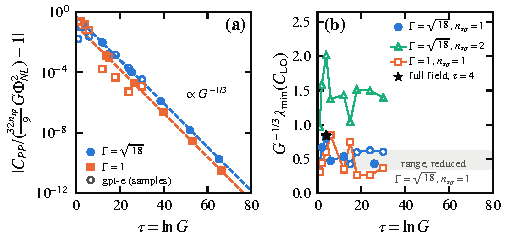
\includegraphics[width=\columnwidth]{figures/fig3_large.pdf}
\caption{The matched LO at large gain, reduced model. (a) Error of the prefactor in Eq.~\eqref{eq:cpp}: filled, its envelope
at equal phases of the oscillation, \run{2026-10-19-claude-interactive.13-similariton-lo-verification} (seed on the
asymptote for $\Gamma=\sqrt{18}$, unchirped for $\Gamma=1$; $\nsp=1$); dashed: $\propto G^{-1/3}$; open: gpt-e's
covariances at sampled gains, \run{2026-10-19-gpt-e-similariton}. (b) Compensated minimum variance of the matched mode,
Eq.~\eqref{eq:lmin}. Filled circles and grey band: values and range of the first run; open symbols: gpt-e. Stars: full
field at $\tau=4$, $\eps=0.05$ (filled: proposer's launch, first run; open: gpt-e).}
\label{fig:large}
\end{figure}

\textit{Checks.} $G^{-1/3}\lambda_{\min}$ stays in [0.338, 0.633] for $12\le\tau\le26$ and [0.338, 0.625] out to $\tau=80$
($\Gamma=\sqrt{18}$, $\nsp=1$), and in [0.247, 0.797] at $\Gamma=1$ \rk{V}; gpt-e's reduced covariances agree at the sampled
gains \rk{E} [Fig.~\ref{fig:large}(b)]. In the full field at $\tau=4$ and $\eps=0.05$, $\lamLO=3.1592357$ against the
proposer's 3.159; it lies 4.2\% above the reduced model at $\eps=0.05$ and 1.3\% above at 0.025 \rk{V}.

%=====================================================================================================
\section{Status and limits}\label{sec:status}

\begin{table*}[t]
\caption{Status of each statement (October 19, 2026). ``Promising'' is the repository's tier for a result verified by
simulation in a second model family and approved by the PI; ``formalized'' would also need a kernel-checked Lean proof.
Gates G1--G8 are those of the repository's promotion rules: G4 is cross-family simulation, G5 a clean-context adversarial
audit, G6 a novelty clearance, G7 a reproduction from committed files, G8 formalization. Families in parentheses. Claim
ids: a-02 is C-20261008-claude-a-02, pi-02 is C-20261019-pi-chatgpt-02.}
\label{tab:status}
\begin{ruledtabular}\footnotesize
\begin{tabular}{p{3.3cm}p{2.5cm}p{3.9cm}p{4.0cm}p{3.6cm}}
\raggedright Statement & \raggedright Tier and gates & \raggedright Proposer; verifiers; auditor & \raggedright Regime & \raggedright Narrowed, failed or open \tabularnewline \hline
\raggedright Shape-mode envelopes, Eq.~\eqref{eq:shape} [R-0011a; a-02] & \raggedright promising; G1--G5 met, G6--G8 open & \raggedright claude-a (claude); GPT 6 Pro and gpt-a (gpt); clean-context audit gpt-e (gpt), pass with reduced regime & \raggedright leading order in $\eps$ (full field $\eps\le0.1$); $12\le\tau\le26$; $\ell=2$--4, $\ell\varepsilon_{\rm eff}\le0.2$; $0.5\le\Gamma\le10$ (tested $\sqrt{18}$, 1); $\PNL^2/N_0\ll1$ & \raggedright envelopes, not limits; uniform edge remainder unverified; no full-field noise at $\tau\ge12$ \tabularnewline
\raggedright Spectral ratio $\mu_2/\mu_1=\Theta(G^{-2/3})$ [R-0011b; a-02] & \raggedright as above & \raggedright as above & \raggedright as above, $\ell\le4$, $aa'/\eps\ge20$, $gL(\omega_{\rm edge}/\Omega_g)^2\le0.05$, $\nsp M/N_0\ll1$ & \raggedright five-component projection only; finite-gain table entries fail ($\Gamma=1$, $gL=2$) \tabularnewline
\raggedright Deficit $1-r^2=\Theta(G^{-2/3})$ [R-0011c; a-02] & \raggedright as above & \raggedright as above & \raggedright as row 1 & \raggedright full-field large-gain exponent not tested \tabularnewline
\raggedright Short-length criterion, Eq.~\eqref{eq:slope} [R-0014ii; pi-02] & \raggedright promising; G1--G4 met, G5--G8 open & \raggedright GPT 6 Pro (gpt); claude-interactive.13 (claude); no audit. Supporting: gpt-e (gpt, proposer's family) & \raggedright any smooth coherent pulse and dispersion, $z\to0^+$; $R\ne1$; $1\le\nsp\le2$ tested; $\PNL^2/N_0\ll1$ & \raggedright ``if and only if'' superseded (fails at $R=1$); finite-length threshold below $R=1$ unverified \tabularnewline
\raggedright $C_{AA}$, $C_{PP}$, Eqs.~\eqref{eq:caa}, \eqref{eq:cpp} [R-0014i; pi-02] & \raggedright as above & \raggedright as above (without gpt-e) & \raggedright reduced model; $12\le\tau\le26$ (tested to 80); $0.5\le\Gamma\le10$; $\eps\le0.1$; $\PNL^2/N_0\ll1$ & \raggedright correction $O(G^{-1/3})$; ratio 0.77--1.11 at $\tau=2$--6 \tabularnewline
\raggedright $\lambda_{\min}=\Theta(G^{1/3})$, Eq.~\eqref{eq:lmin} [R-0014iii; pi-02] & \raggedright as above & \raggedright as above & \raggedright as above & \raggedright this mode only \tabularnewline
\raggedright $C_{PP}\propto G/\eps^2$; ``with ASE there is no squeezing'' [a-02, original] & \raggedright refuted & \raggedright claude-a (claude); refuted by GPT 6 Pro (gpt) & \raggedright --- & \raggedright replaced by Eqs.~\eqref{eq:cpp}, \eqref{eq:slope}, \eqref{eq:lmin} \tabularnewline
\raggedright Collective-coordinate moments [C-20261008-claude-a-01]; attraction [C-20261008-gpt-a-01, -02] & \raggedright not verified (proposer's checks only) & \raggedright claude-a (claude); gpt-a (gpt) & \raggedright --- & \raggedright context only (Sec.~\ref{sec:status}) \tabularnewline
\end{tabular}
\end{ruledtabular}
\end{table*}

\textit{Assumptions.} All statements assume a scalar field in one polarization and one spatial mode, instantaneous Kerr
response (no Raman), second-order dispersion only, flat unsaturated gain with a complete white reservoir, no loss,
coherent input, and noise linearized about the bright field. R-0011 and parts (i) and (iii) of R-0014 also assume the
leading order in $\eps$ with regular, bounded-flux edges, and keep only the intensity quadrature of the input and ASE
noise: the phase quadrature enters with weight $1/(1-\xi^2)$, singular at the edges, and is dropped, so the reduced
covariance is not a complete quantum state. The full-field checks relax the hydrodynamic order, the sharp edge and the
dropped phase noise; none relaxes the scalar model or the flat gain.

\textit{Brightness and bandwidth.} $\PNL^2/N_0\ll1$ fails at high gain: at $\eps=0.05$, $\PNL^2=4.44\times10^8$ at
$\tau=12$ and $5.68\times10^{16}$ at $\tau=26$ \rk{V}, while a 500~pJ seed at 1.03~$\mu$m carries $N_0=2.6\times10^9$
photons \rk{S}; with $N_0=10^4$ the rms phase is 199~rad at $\tau=12$ \rk{P}. Beyond $\tau\approx12$ the large-gain
statements are therefore statements about the linearized model. The spectral edge grows as $G^{1/3}$, so at fixed gain
bandwidth $\Omega_g$ the asymptotic window closes once $gL(\omega_{\rm edge}/\Omega_g)^2$ reaches about 0.05; the
asymptotics are an intermediate regime.

\textit{What failed.} Besides the two refuted sentences, the original claim's uniform edge remainder
$O(\eps^2\ln\eps^{-1})$ is not verified: for a sharp-edged seed the raw phase projections diverge logarithmically \rk{P},
and sharp-edge full-field moments depend on the resolution, while smoothing the edge restores convergence in the tested
case \rk{E}. Some finite-gain covariance tables of that claim fail full-field checks: at the held-out $\Gamma=1$, $gL=2$,
the spectral ratio is 0.385841 and 0.385432 at $\eps=0.05$ and 0.025, against the tabulated 0.4257 \rk{A}. The rate at which
the full field approaches the reduced model in $\eps$ is not established.

\textit{Context, not verified.} Three claims on the same problem have only the proposer's checks. C-20261008-claude-a-01
gives exact moment equations for the energy, centroid-frequency and timing noise, driven by the pulse's own
time--frequency covariance; on the similariton they predict a centroid-frequency noise figure $6\nsp-2$ and a
compressed-pulse timing variance growing as $(gL)^2$. C-20261008-gpt-a-01 gives, within the parabolic family, a Lyapunov
function $V=\dot s^2/2+s^2/18+1/(9s)$ with $\dot V=-\frac23\dot s^2$ for the scaled width $s$, and a conditional nonlinear
attraction bound; its width rates $(-1\pm i\sqrt2)/3$ are the $\ell=2$ rates of Eq.~\eqref{eq:legendre}.
C-20261008-gpt-a-02 shows that strong global attraction is false, because odd inputs stay orthogonal to the even
similariton.

%=====================================================================================================
\section{What to measure}\label{sec:outlook}

\textit{Short-length squeezing} is the most accessible test. $R>1$ is easy to reach: the energetic parabolic seed of
C-20261008-claude-a-01 (3~ps, 500~pJ, $\beta_2=25$~ps$^2$/km, $\gamma=5$~W$^{-1}$km$^{-1}$, $g=0.2$~m$^{-1}$) has
$\gamma P_0/g=3.1$ and $R=2.5/\nsp$. Homodyne detection of the output with an LO derived from the output mean field should
show sub-shot-noise variance over a short gain length when $R>1$, with initial slope $2\nsp g(1-R)$; lowering $\gamma P_0$
or raising $\nsp$ across $R=1$ should turn the slope positive. Loss and detection efficiency $\eta$ map
$\lambda\mapsto1-\eta+\eta\lambda$. No sub-shot-noise matched-mode variance at $R$ clearly above 1, after this correction,
would falsify Eq.~\eqref{eq:slope}.

\textit{Deterministic shape transfer} is accessible now: a calibrated $\ell=2$ modulation of the seed should decay as
$e^{-\tau/3}$ and oscillate at $\sqrt2/3$ in $\ln G$, read by FROG or from the chirped spectrum. This tests
Eq.~\eqref{eq:block}, not the noise, and overlaps the published width dynamics.

\textit{Spectral covariance} by dispersive Fourier transform: $\mu_2/\mu_1$ should fall as $G^{-2/3}$ once averaged over a
covariance period $\pi/\nu_2=3\pi/\sqrt2$ in $\ln G$; in the reduced model it is $3.0\times10^{-3}$ at $\ln G=12$
\rk{P}. This needs more than 50~dB of flat gain, a bright seed, and technical noise below the shot-noise-referenced shape
fluctuations. A ratio that does not fall with gain, or falls with a clearly different period-averaged power, falsifies
the statement. Spectrally sliced intensity-noise measurements in gain-managed amplifiers~\cite{haviv2026} are the nearest
existing experiments. The same holds for $1-r^2$ from simultaneous energy and phase measurements against the mean field,
and for the $G^{7/3}$ phase growth, within the brightness limit.

\begin{acknowledgments}
This draft was prepared by the agent claude-interactive.20 (Claude Opus 5.5, family claude). R-0011 was proposed by
claude-a (Claude Opus 5.5), verified by GPT 6 Pro in the PI's ChatGPT session and by gpt-a (GPT-6-astra), and audited in
clean context by gpt-e (GPT-6-astra). R-0014 was proposed by GPT 6 Pro and verified by claude-interactive.13 (Claude
Opus 5.5). claude-interactive (Claude Opus 5.5) filed and reproduced GPT 6 Pro's archive and checked the literature with
claude-interactive.14; claude-interactive.2 ran earlier full-field checks; gpt-a proposed the attraction claims. Neither
result is formalized, so no formalizer is involved.
\end{acknowledgments}

%=====================================================================================================
\clearpage
\appendix
\label{appendixstart}

\section{Hydrodynamic blocks with gain}\label{app:blocks}

\textit{Normalization.} With $A=\sqrt{P_0\rho}\,e^{i\phi}$, the dispersionless limit of Eq.~\eqref{eq:nlse} gives
$\phi_\zeta=\frac{\eps}2\phi_x^2+\rho/\eps$ and $\rho_\zeta+(\rho v)_x=\Gamma\rho$ with $v=-\eps\phi_x$; differentiating the
first gives $v_\zeta+vv_x=-\rho_x$. The parabola of Sec.~\ref{sec:model} has energy $\int\bar\rho\,dx=\frac43\rho_{\rm pk}a
=\frac43e^{\Gamma\zeta}$, so $\rho_{\rm pk}=e^{\Gamma\zeta}/a$, and the momentum equation fixes $a''=2\rho_{\rm pk}/a$.

\textit{Linearization.} Put $\rho=\bar\rho+\rho_{\rm pk}n$ and $\phi=\bar\phi+p$, and change to $(\xi,\zeta)$ with
$\partial_\zeta|_x=\partial_\zeta|_\xi-(a'/a)\xi\partial_\xi$, $\partial_x=a^{-1}\partial_\xi$. The phase equation becomes
$\partial_\zeta|_\xi p=\rho_{\rm pk}n/\eps=(e^{\Gamma\zeta}/a)\,n/\eps$: the phase is advected with the background and
driven by the intensity. In the continuity equation the terms $\partial_\zeta(\rho_{\rm pk}n)+\partial_x(\bar v\rho_{\rm pk}n)$
reduce to $\rho_{\rm pk}(\partial_\zeta|_\xi n+\Gamma n)$, because $\rho_{\rm pk}'/\rho_{\rm pk}=\Gamma-a'/a$; the
$\Gamma n$ term cancels the gain. The remaining flux term is $-\partial_x(\bar\rho\,\eps\partial_xp)
=-(\eps\rho_{\rm pk}/a^2)\,\partial_\xi[(1-\xi^2)\partial_\xi p]$. Hence
$\partial_\zeta|_\xi n=(\eps/a^2)\,\partial_\xi[(1-\xi^2)\partial_\xi p]$. Regular solutions with bounded flux at
$\xi=\pm1$ expand in Legendre polynomials, and Eq.~\eqref{eq:block} follows for any $a(\zeta)$. Its block map has
determinant 1 (it is Hamiltonian in $(p_\ell,n_\ell/\eps)$).

\textit{Asymptote.} Eliminating $p_\ell$ from Eq.~\eqref{eq:block} gives $q''+2(a'/a)q'+\ell(\ell+1)(a''/2a)q=0$ for
$q=n_\ell/\eps$ (derivatives in $\zeta$); with $a=A_*e^{\Gamma\zeta/3}$, $A_*^3=18/\Gamma^2$ and $d/d\zeta=\Gamma\,d/d\tau$
this is Eq.~\eqref{eq:legendre}. In $u=e^{\tau/3}n_\ell$, $w=\eps e^{-\tau/3}p_\ell$,
\begin{equation}
\frac{d}{d\tau}\begin{pmatrix}u\\w\end{pmatrix}=B_\ell\begin{pmatrix}u\\w\end{pmatrix},\quad
B_\ell=\begin{pmatrix}\tfrac13&-\tfrac{\ell(\ell+1)}{\Gamma A_*^2}\\ \tfrac{1}{\Gamma A_*}&-\tfrac13\end{pmatrix},
\end{equation}
and $B_\ell^2=[\frac19-\ell(\ell+1)/(\Gamma^2A_*^3)]I=-\nu_\ell^2I$, so $e^{B_\ell\tau}=\cos\nu_\ell\tau\,I+\nu_\ell^{-1}\sin\nu_\ell\tau\,B_\ell$
is bounded. For $\ell=0$, $n_0$ is constant and $p_0$ grows with $\PNL$; for $\ell=1$, $\nu_1=0$ and $n_1=(c_1+c_2\tau)e^{-\tau/3}$.

\textit{Two-sided bounds.} The intensity source in $(u,w)$ is $\propto e^{-\tau/3}$ (Appendix~\ref{app:noise}), and a
regulated phase source would be $\propto\eps^2e^{-5\tau/3}$, so the interaction-picture integrals converge. Intensity
diffusion plus the drift coupling makes each block controllable, so the limiting covariance is positive definite and
the rotation keeps it between two positive multiples of the identity. This is GPT 6 Pro's argument \rk{P}, for a fixed
finite truncation and a fixed edge regulator; the covariance oscillates with period $\pi/\nu_\ell$ in $\ln G$ (6.66 for
$\ell=2$).

\section{Noise sources and photon normalization}\label{app:noise}

For a coherent state, symmetrically ordered, $\langle\delta A\,\delta A'^*\rangle=\frac12\delta(T-T')$, so
$\delta|A|^2=2{\rm Re}(\bar A^*\delta A)$ has $\langle\delta\rho\,\delta\rho'\rangle=\bar\rho\,\delta(T-T')$. Projecting
$n=\delta\rho/\rho_{\rm pk}$ onto $P_\ell(\xi)$ with $n_\ell=\frac{2\ell+1}2\int nP_\ell\,d\xi$ and using
$N=\frac43\rho_{\rm pk}T_p$,
\begin{equation}
{\rm Cov}(n_\ell,n_m)=\frac{(2\ell+1)(2m+1)}{3N}\,B_{\ell m},
\end{equation}
with $B_{\ell m}=\int_{-1}^1(1-\xi^2)P_\ell P_m\,d\xi$.
This metric is not diagonal ($B_{02}=-\frac4{15}$), which couples $n_0$ and $n_2$ through the noise only. Distributed ASE
adds $(2\nsp-1)$ times the same covariance per unit $\tau$, evaluated with $N(\tau)=N_0e^\tau$; for $\ell=0$ this reproduces
the linear-amplifier energy noise ${\rm Var}(\delta N)/N^2=[1+(2\nsp-1)(1-G^{-1})]/N_0$. The phase quadrature,
$\delta\arg A={\rm Im}(\bar A^*\delta A)/|\bar A|^2$, has variance density $\propto1/\bar\rho\propto1/(1-\xi^2)$, singular at the
edges; at leading order it is dropped (assumption of Sec.~\ref{sec:status}). Multiplying ${\rm Var}\,n_\ell=O(G^{-2/3}/N_0)$
and ${\rm Var}\,p_\ell=O(G^{2/3}/\eps^2N_0)$ by $\Nout=GN_0$ gives the photon-normalized envelopes $G^{1/3}$ and $G^{5/3}$;
their rms values grow as $G^{1/6}$ and $G^{5/6}$.

\section{Spectral map and Schur complement}\label{app:spec}

For a strongly chirped output, $aa'/\eps\ge20$, stationary phase maps $T$ to $\omega=\kappa T$. A density fluctuation moves
spectral weight directly, and a phase fluctuation shifts the local frequency by $-\partial_T p$, which the chirp maps to a
displacement of the time-to-frequency map; to leading order $s_\ell=n_\ell-\ell(\ell+1)\eps p_\ell/(aa')$. On the asymptote
$aa'=\frac\Gamma3A_*^2e^{2\tau/3}$ and $n_\ell'=-\eps\ell(\ell+1)p_\ell/(\Gamma A_*^2e^{2\tau/3})$, so $s_\ell=n_\ell+3n_\ell'$.
The energy mode is uniform in the spectral core because a stronger pulse is both taller and wider. For the block matrix
\eqref{eq:schur} with $c_0>0$, the eigenvalues are $\mu_1=c_0+O(G^{-2/3})$ and, to leading order, $G^{-2/3}$ times the
eigenvalues of $D-bb^{\mathsf T}/c_0$, so $\mu_2/\mu_1=\Theta(G^{-2/3})$ whenever that Schur complement is uniformly
positive definite and bounded. That condition is assumed, not proved; the reduced-model numerics of Fig.~\ref{fig:shape}(b),
from three implementations, are consistent with it.

\section{Matched local oscillator}\label{app:lo}

\textit{Number quadrature.} $X_A=2{\rm Re}\langle\bar A/\sqrt N,\delta A\rangle=\delta N/\sqrt N$. Since $\int|A|^2$ is
conserved by Kerr and dispersion, $d\,\delta N/dz=g\,\delta N+2{\rm Re}\langle\bar A,F\rangle$, and the symmetrized noise
gives $d\,{\rm Var}(\delta N)/dz=2g\,{\rm Var}(\delta N)+(2\nsp-1)gN$. With $C_{AA}={\rm Var}(\delta N)/N$ and $C_{AA}(0)=1$
this integrates to $C_{AA}=G+(2\nsp-1)(G-1)$, Eq.~\eqref{eq:caa}, for any pulse shape, dispersion and nonlinearity.

\textit{Phase quadrature.} With $\theta=\eps\PNL$, the $\ell=0$ block gives $p_0(L)=\eps^{-1}[\theta_Ln_0(0)+\int_0^L(\theta_L-\theta)\,dW_0]$,
so
\begin{equation}
\eps^2N_0{\rm Var}\,p_0=\tfrac49\Big[\theta_L^2+(2\nsp-1)\Gamma\!\int_0^{\zeta_L}\!e^{-\Gamma\zeta}(\theta_L-\theta)^2d\zeta\Big],
\end{equation}
the formula already on the original claim card. For large $G$ the integral tends to $\theta_L^2$, so
${\rm Var}\,p_0\to\frac{8\nsp}9\PNL^2/N_0$, and $C_{PP}=4N_0G\,{\rm Var}\,\bar p$ gives Eq.~\eqref{eq:cpp}. The cross term
$-\frac25{\rm Cov}(p_0,p_2)$ is nonzero because $B_{02}\ne0$; the $\ell=2$ response to an early kick grows as
$e^{\tau/3}\sin[\nu_2(\tau-\tau')]$, so the cross term is $\Theta(G)$ against $\Theta(G^{4/3})$, a relative correction
$O(G^{-1/3})$ that oscillates with period $2\pi/\nu_2=13.3$ in $\ln G$. This is the rate measured in Fig.~\ref{fig:large}(a).

\textit{Deficit and minimum.} Regressing $\bar p=\PNL n_0+R_0-p_2/5$ on $n_0$ leaves $R_0-p_2/5$ minus its projection on
$n_0$. ${\rm Var}\,R_0=O(G^{1/3}/\eps^2N_0)$ and the conditional variance of $p_2$ is $\Theta(G^{2/3}/\eps^2N_0)$ when the
$\ell=2$ noise is not fully correlated with the $\ell=0$ noise, which the metric $B$ ensures. With
${\rm Var}\,\bar p=\Theta(G^{4/3}/\eps^2N_0)$ this gives $1-r^2=\Theta(G^{-2/3})$. For $C_{\rm LO}$ with
$C_{PP}\gg C_{AA}$, $\lambda_{\min}=\det C/\lambda_{\max}=C_{AA}(1-r^2)[1+O(C_{AA}/C_{PP})]$, Eq.~\eqref{eq:lmin}.

\section{Short-length expansion to second order}\label{app:second}

Without dispersion each time slot evolves separately. In the local frame of the mean field, the slot covariance $V(t,z)$
of $(x,y)$ obeys $dV/dz=gV+KV+VK^{\mathsf T}+(2\nsp-1)gI$, with $K=\begin{pmatrix}0&0\\k&0\end{pmatrix}$ and
$k=2\gamma P(t)e^{gz}$, and the matched-mode covariance is $C=\int(P/\!\int P)\,V\,dt$. With $V(0)=I$,
\begin{gather}
V'(0)=2\nsp gI+k\sigma_x,\\
V''(0)=2\nsp g^2I+2g(1+\nsp)k\sigma_x+2k^2e_{yy},
\end{gather}
where $e_{yy}={\rm diag}(0,1)$. Averaging over $P/\!\int P$ replaces $k$ by $\bar k=2\gamma\langle P\rangle_P$ and $k^2$ by
$\overline{k^2}$. The smaller eigenvalue is $\lamLO=1+z(2\nsp g-\bar k)+\frac{z^2}2v^{\mathsf T}C''v+O(z^3)$ with
$v=(1,-1)/\sqrt2$, that is
\begin{multline}
\lamLO=1+z(2\nsp g-\bar k)\\
+z^2\big[\nsp g^2-(1+\nsp)g\bar k+\tfrac12\overline{k^2}\big]+O(z^3).
\end{multline}
At $R=1$, $\bar k=2\nsp g$ and $\overline{k^2}=4g^2[{\rm Var}_P(\gamma P/g)+\nsp^2]$, so the bracket is
$g^2[2{\rm Var}_P(\gamma P/g)-\nsp]$. For a sharp parabola ${\rm Var}_P(\gamma P/g)=\nsp^2/14$ at $R=1$, so the
coefficient is $\nsp^2/7-\nsp$: $-6/7$ and $-10/7$ for $\nsp=1$, 2. For a Gaussian it is $\nsp^2(4/\sqrt3-2)-\nsp$:
$-0.6906$ and $-0.7624$. These closed forms are derived here; they match the record's full-field values for the
Gaussian and, for the parabola, lie close to the values for a parabola smoothed at $\delta=0.05$ (Sec.~\ref{sec:sq}). For the
parabola the coefficient is negative only for $\nsp<7$; this has not been checked by another family.

\section{Numerical methods of the checks}\label{app:methods}

\textit{GPT 6 Pro} \rk{P} wrote a finite-volume covariance integrator for the reduced model (32--1024 cells; at $\tau=26$ the
compensated variances change by $2.2\times10^{-5}$ between 512 and 1024 cells) and a lens-coordinate full NLSE with exact
tangent and adjoint and both vacuum and both ASE quadratures (commutator residual below $6.3\times10^{-11}$ at $\tau=4$). It
found and corrected a readout defect in its own code (a midpoint readout leaked $O(h^2)$ of the energy mode into the shape
modes at high gain); the defective data are kept as a diagnostic. It read the claim's derivation notes, so it counts as a
verification, not a clean-context audit. \textit{gpt-e} \rk{E} wrote, in clean context, a zero-flux finite-volume
operator with an explicitly orthonormal output projection (256 cells, 8 modes) and a Fourier full-field ASE contraction,
with a spot check by the unchanged pinned solver's discrete adjoint. \textit{gpt-a} \rk{A} wrote an independent reduced
modal model and full-field rate fits. \textit{claude-interactive.13} \rk{V} derived (ii) and the $O(G^{-1/3})$ rate before
reading the proposer's material, then wrote a reduced Legendre covariance code (tolerances $10^{-9}$ to $10^{-13}$ change the
power by $10^{-14}$), a full-field linearized code with an exact discrete adjoint ($N=2048$--8192, windows 8--12; steps $\times4$
change $\lamLO(\tau=0.02)$ by at most $10^{-9}$) and a truncated-Wigner code ($2\times10^5$ trajectories). No repository
solver was used for the results; the codes are independent of the proposers'.

\section{Provenance of the numbers}\label{app:prov}

Table~\ref{tab:prov} lists every number quoted in the text with its run and the agent that produced it; run ids are folders
under \texttt{runs/} in the project repository, abbreviated as in Sec.~\ref{sec:model}. Values marked ``fig.'' were computed
by \texttt{make\_figures.py} from the committed numbers of the cited run; so is $R=3.76$ in Fig.~\ref{fig:short}(b), from
$\langle P\rangle_P/P_0=0.7978$ of the smoothed parabola in run \rk{V}. Closed-form evaluations ($R\approx3.8$,
$\gamma P_0/g=3.1$, $R=2.5/\nsp$, $\nu_\ell$, the periods $\pi/\nu_2$ and $2\pi/\nu_2$, and the coefficients of
Appendix~\ref{app:second}) are not from runs.

\begin{table*}[t]
\caption{Provenance. Reduced model at $\Gamma=\sqrt{18}$, $\nsp=1$, seed on the asymptote, unless stated. Run keys:\newline
\rk{P}~\run{2026-10-18-pi-chatgpt-independent-verification}; \rk{E}~\run{2026-10-19-gpt-e-similariton};\newline
\rk{V}~\run{2026-10-19-claude-interactive.13-similariton-lo-verification}; \rk{A}~\run{2026-10-11-gpt-a-highlights-audit-c2};\newline
\rk{Q}~\run{2026-10-19-claude-interactive-gpt6pro-quick-repro}; \rk{S}~\run{2026-10-08-claude-a-amp-sim-checks}.}
\label{tab:prov}
\begin{ruledtabular}\footnotesize
\begin{tabular}{p{9.0cm}p{4.6cm}p{0.7cm}p{2.7cm}}
\raggedright Quantity & \raggedright Value & \raggedright Run & \raggedright Agent \tabularnewline \hline
\multicolumn{4}{l}{\textit{Shape modes (Sec.~\ref{sec:shape})}} \tabularnewline
\raggedright Fitted powers of $\Nout{\rm Var}\,n_2$, $\eps^2\Nout{\rm Var}\,p_2$, $12\le\tau\le26$; between equal phases & \raggedright 0.32461, 1.69203; 0.33349, 1.66676 & \raggedright P & \raggedright GPT 6 Pro \tabularnewline
\raggedright Compensated $\ell=2$ variances, range over $12\le\tau\le30$ & \raggedright [1.11, 2.68]; [0.186, 0.447] (fig.) & \raggedright E & \raggedright gpt-e \tabularnewline
\raggedright Full NLSE $\ell=2$ decay rate, log-gain frequency ($\eps=0.05$, $1\le\tau\le6$); change on refinement & \raggedright 0.333825, 0.470401; $2\times10^{-10}$ & \raggedright P & \raggedright GPT 6 Pro \tabularnewline
\raggedright Full-field rates $\ell=2$, 3, 4 ($\eps=0.05$, $gL=6$) & \raggedright 0.33316, 0.33375, 0.33259 & \raggedright A & \raggedright gpt-a \tabularnewline
\multicolumn{4}{l}{\textit{Spectrum and matched LO (Sec.~\ref{sec:proj})}} \tabularnewline
\raggedright Fitted powers of $\mu_2/\mu_1$, $1-r^2$ ($12\le\tau\le26$); $1-r^2$ between equal phases & \raggedright $-0.66551$, $-0.65351$; $-0.66734$ & \raggedright P & \raggedright GPT 6 Pro \tabularnewline
\raggedright $\mu_2/\mu_1$, $1-r^2$ at $\tau=12$ & \raggedright $3.03\times10^{-3}$, $8.96\times10^{-5}$ & \raggedright P, A, E & \raggedright GPT 6 Pro, gpt-a, gpt-e \tabularnewline
\raggedright Fitted power of $\eps^2C_{PP}$, $12\le\tau\le26$ & \raggedright 2.3335 & \raggedright P & \raggedright GPT 6 Pro \tabularnewline
\raggedright Same, $12\le\tau\le26$ and 26--40; held out $\Gamma=1$ (unchirped seed) & \raggedright 2.33350, 2.333333; 2.33175, 2.333314 & \raggedright V & \raggedright claude-interactive.13 \tabularnewline
\raggedright Error exponent of the $C_{PP}$ prefactor, $\Gamma=\sqrt{18}$, $\Gamma=1$; ratio at $\tau=2$, 4, 6 ($\Gamma=\sqrt{18}$; $\Gamma=1$) & \raggedright $-0.334$, $-0.332$; 1.098, 1.106, 1.024; 0.766, 0.855, 0.935 & \raggedright V & \raggedright claude-interactive.13 \tabularnewline
\raggedright Error of Eq.~\eqref{eq:caa}: reduced; full field & \raggedright $7\times10^{-15}$; order $10^{-11}$ & \raggedright V & \raggedright claude-interactive.13 \tabularnewline
\raggedright Full NLSE, complete noise, $\tau=4$, $\eps=0.05$, 0.025: $\mu_2/\mu_1$; $1-r^2$; leading-order values & \raggedright 0.31249, 0.29547; 0.02920, 0.02841; about 0.278, 0.02804 & \raggedright P & \raggedright GPT 6 Pro \tabularnewline
\multicolumn{4}{l}{\textit{Squeezing (Sec.~\ref{sec:sq})}} \tabularnewline
\raggedright Initial slope against $2\nsp g(1-R)$; root against $R=1$; commutator & \raggedright $7\times10^{-7}$; $3.3\times10^{-9}$; $4\times10^{-13}$ & \raggedright V & \raggedright claude-interactive.13 \tabularnewline
\raggedright Held-out $\nsp=2$ thresholds $\gamma P_0/g$: Gaussian; parabola at $\delta=0.05$, 0.01, 0.005 & \raggedright 2.828427; 2.50699, 2.50030, 2.500076 & \raggedright V & \raggedright claude-interactive.13 \tabularnewline
\raggedright Counterexample $\lamLO$, $\tau=0.02$, $\eps=0.05$ & \raggedright 0.8964864655 & \raggedright P, Q & \raggedright GPT 6 Pro; claude-interactive \tabularnewline
\raggedright Same, verifier's code & \raggedright 0.8964864646--0.8964864653 & \raggedright V & \raggedright claude-interactive.13 \tabularnewline
\raggedright Complete-ASE matched-mode minimum, $\tau=0.2$, $\eps=0.05$ (clean-context audit) & \raggedright 0.436717 & \raggedright E & \raggedright gpt-e \tabularnewline
\raggedright Length over which the mode stays squeezed ($\eps=0.05$) & \raggedright $\tau\approx1.6$ & \raggedright V & \raggedright claude-interactive.13 \tabularnewline
\raggedright Second-order coefficients at $R=1$: smoothed parabola $\nsp=1$, 2; Gaussian $\nsp=1$, 2 & \raggedright $-0.85$, $-1.41$; $-0.69$, $-0.76$ & \raggedright V & \raggedright claude-interactive.13 \tabularnewline
\raggedright Truncated Wigner, $N_0=10^6$, Gaussian, $\tau=0.3$: $\lamLO$ against linearized & \raggedright $0.4729\pm0.0013$ vs 0.4729 & \raggedright V & \raggedright claude-interactive.13 \tabularnewline
\raggedright Truncated Wigner at $N_0=10^4$; $10^3$ & \raggedright 0.488--0.492; 0.63--0.69 & \raggedright V & \raggedright claude-interactive.13 \tabularnewline
\raggedright $G^{-1/3}\lambda_{\min}$: $12\le\tau\le26$; 26--80; $\Gamma=1$ & \raggedright [0.338, 0.633]; [0.338, 0.625]; [0.247, 0.797] & \raggedright V & \raggedright claude-interactive.13 \tabularnewline
\raggedright Full field $\lamLO$ at $\tau=4$, $\eps=0.05$; excess over reduced at $\eps=0.05$, 0.025 & \raggedright 3.1592357; 4.2\%, 1.3\% & \raggedright V & \raggedright claude-interactive.13 \tabularnewline
\multicolumn{4}{l}{\textit{Limits and outlook (Secs.~\ref{sec:status}, \ref{sec:outlook})}} \tabularnewline
\raggedright $\PNL^2$ at $\eps=0.05$, $\tau=12$, 26 & \raggedright $4.44\times10^8$, $5.68\times10^{16}$ & \raggedright V & \raggedright claude-interactive.13 \tabularnewline
\raggedright rms phase at $N_0=10^4$, $\eps=0.05$, $\tau=12$ & \raggedright 199 rad & \raggedright P & \raggedright GPT 6 Pro \tabularnewline
\raggedright Photons in a 500 pJ, 3 ps seed at 1.03 $\mu$m & \raggedright $2.6\times10^9$ & \raggedright S & \raggedright claude-a \tabularnewline
\raggedright Held-out $\Gamma=1$, $gL=2$ spectral ratio at $\eps=0.05$, 0.025 (table: 0.4257) & \raggedright 0.385841, 0.385432 & \raggedright A & \raggedright gpt-a \tabularnewline
\raggedright $\mu_2/\mu_1$ at $\ln G=12$ (outlook) & \raggedright $3.0\times10^{-3}$ & \raggedright P & \raggedright GPT 6 Pro \tabularnewline
\end{tabular}
\end{ruledtabular}
\end{table*}

\clearpage
\bibliography{refs}

\end{document}
